\chapter{Discussion and conclusions}

\tab Based on the experimental results , we can affirm that a significant number of structural dependencies are also logical \cite{ct10}, \cite{ct9}.The number of overlaps between structural and logical dependencies is influenced by the rules of extracting logical dependencies. In average, if we choose to take into consideration all commits without setting a threshold for the number of files changed we obtain an overlap of structural and logical dependencies of 71\% which is with 47\% more than if we take into consideration only commits with less then 5 source code files changed per commit (Figure \ref{fig:figvenn}). \\ It can be observed that at extremities we have systems ID 5,6 with an overlap only 2\% and system ID 2 with an overlap of 100\%. However this systems are very small, but the other systems, that have more commits and more classes, have close rates of overlapping.
\begin{figure}[h]
\centering
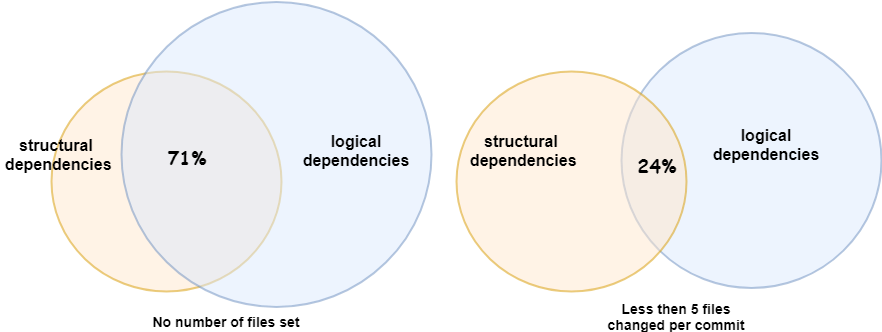
\includegraphics[scale=0.6]{fig4.png}
\caption{Venn diagrams of the overlapping rates with comments taken into consideration as change}
\label{fig:figvenn}
\end{figure}


Table \ref{table:13} illustrates the percentage rates for all the categories mentioned without filtering the logical dependencies occurrences, in addition a last category that takes all commits regardless of the number of changed files was introduced. How it can be seen, the overlapping rates are also influenced by the comments filtering. The rates are with aprox 6\% lower if comments are not taken into consideration as a change. 


\begin{table}
  \centering
  \begin{tabular}{@{}c||cc@{}}
    \toprule
       Category & With comments & Without comments  \\
    \midrule
less 5	&	19,7\% &	18,9\%	\\
more 5 less 20	&	31,19\% &	28,7\%\\
more 20	&	31,47\%	&	29,43\%\\
total & 60,4\% &57,28\% \\
    \bottomrule
  \end{tabular}
  \caption{ Overall percentage rates without filtering the logical dependencies occurrences.}
   \label{table:13}
\end{table}

Table \ref{table:14}  illustrates the percentage rates for all the categories mentioned by filtering the logical dependencies occurrences, in addition a last category that takes all commits regardless of the number of changed files was introduced. How it can be seen, the overlapping rates are lower with 50\% compared with table \ref{table:13} . This indicates that a lot of logical dependencies are the result of a single commit in which the two elements of the dependency where changed together.


\begin{table}
  \centering
  \begin{tabular}{@{}c||cc@{}}
    \toprule
       Category & With comments & Without comments  \\
    \midrule
less 5	&	9,09\% &	8,67\%	\\
more 5 less 20	&	15,87\% &	13,29\%\\
more 20	&	18,8\%	&	16,52\%\\
total &39,1\% & 35,38\% \\
    \bottomrule
  \end{tabular}
  \caption{Overall percentage rates by filtering the logical dependencies occurrences. }
   \label{table:14}
\end{table}

As a conclusion, it results that large number of structural dependencies are not doubled by logical, which can indicate that the systems are stable. It also results that taken or not comments as change, the final results are not influenced in a big percentage. What influences the result of the overlapping between logical and structural dependencies is the number of files that participate in a commit taken into consideration and the logical dependencies filtering after the number of occurrences.\\
Filtering after the number of occurrences may be a good method but only if the projects are relatively big and have a significant number of commits (example project 18) . Also, setting a big threshold for the number of files taken into consideration can lead to a lot of logical dependencies that are not so relevant, setting a relatively small threshold for the number of files taken into consideration (5 10) can lead to more accurate results since it can filter cases such as branch merge or folder rename that introduce redundant logical dependencies.\\
\tab For future work, we will investigate the cause for the large number of logical dependencies which are not overlapping with structural dependencies.